\section{Method}
\label{sec:method}

This section describes the counting system and the instrument we use to measure it. The
pipeline is deliberately conventional; the measurement is not, and it is what makes the
paper's central result visible.

\subsection{Counting pipeline}
\label{sec:pipeline}

\begin{figure*}[t]
  \centering
  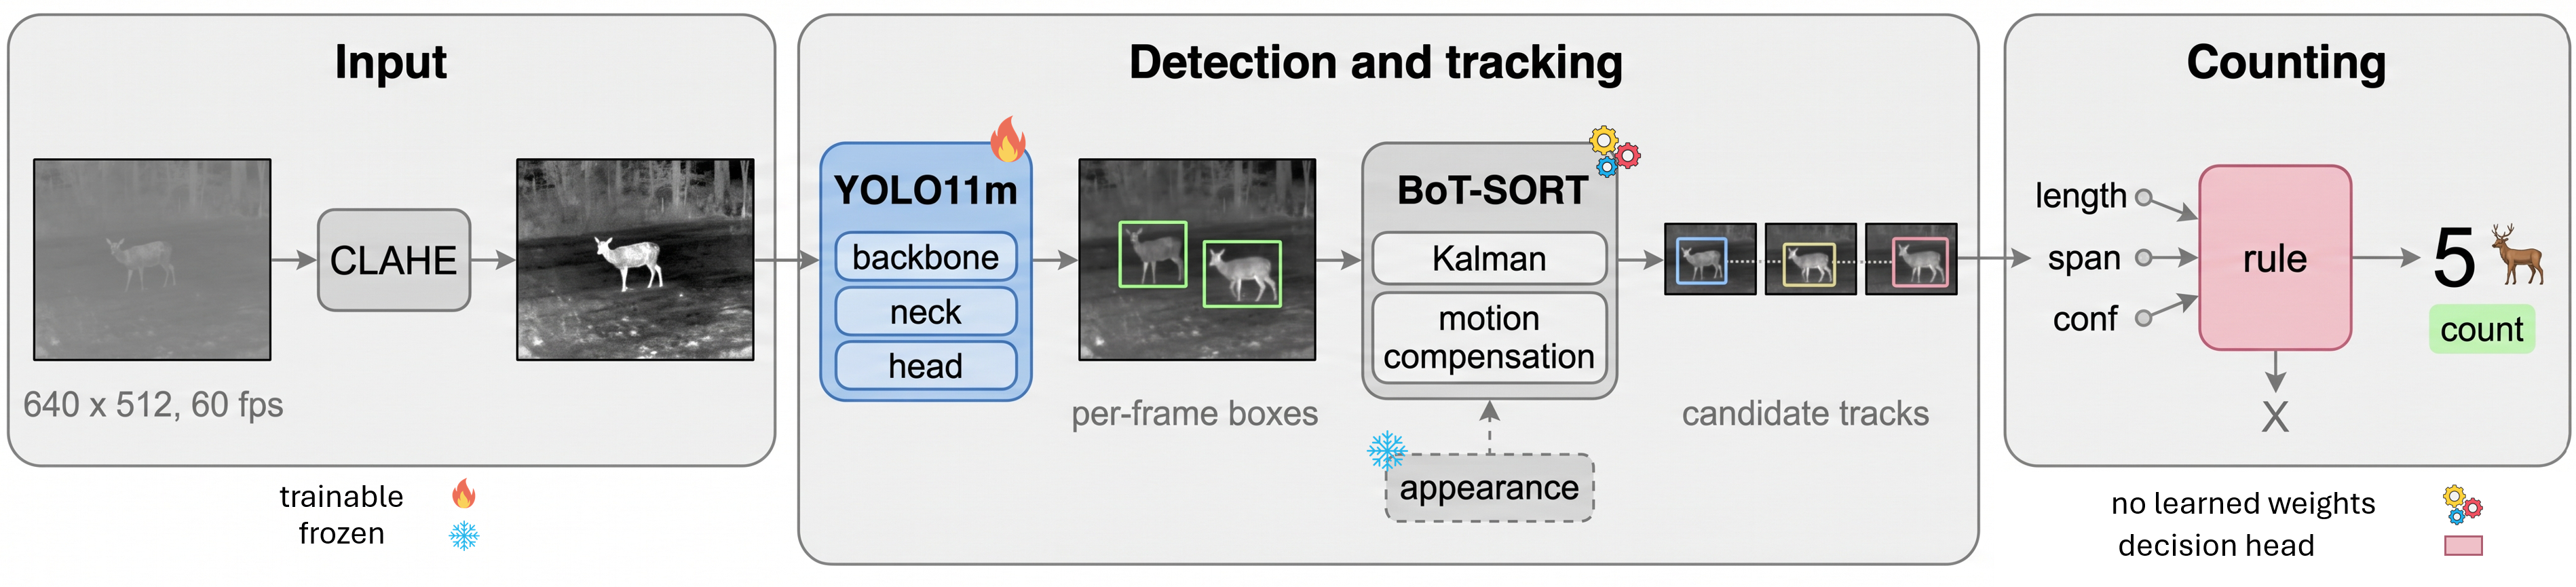
\includegraphics[width=\linewidth]{figures/wildlife_pipeline.png}
  \caption{\textbf{Counting pipeline.} Thermal frames are contrast-normalized, detected
  per frame by YOLO11m, associated into candidate tracks by BoT-SORT with global motion
  compensation, and filtered by a three-parameter confirmation rule; the count is the number
  of accepted tracks. The detector is the only gradient-trained component; the
  tracker's Kalman filter, motion compensation and association carry no weights at all; the
  optional appearance term (dashed) is frozen, reusing the detector's backbone features; and
  the confirmation rule has three parameters fitted by grid search rather than by training. The frames shown
  are illustrative; animals in the corpus are a median $29\times24$\,px
  (\cref{fig:dataset}).}
  \label{fig:pipeline}
\end{figure*}



\Cref{fig:pipeline} shows the system. Detections from YOLO11m at 640\,px are associated by
BoT-SORT~\cite{aharon2022botsort} with
sparse-optical-flow global motion compensation --- mandatory here, since the whole frame
translates as the vehicle moves --- producing candidate tracks. A confirmation stage then
decides which candidates are real, distinct animals. The count is the number of accepted
candidates.

The confirmation baseline is a three-parameter rule: accept a candidate if it persists for
at least $m$ frames, spans at least $s$ seconds, and the mean of its five highest
per-frame detector confidences is at least $c$. Under the held-out protocol
(\cref{sec:heldout}) the swept values are $m\ge20$, $s\ge0$, $c\ge0.65$.

We additionally recover \emph{orphan} detections --- those the tracker returns without a
track identity --- by linking detections within a temporal gap and a scale-normalized
distance into pseudo-tracks. Without this, single-frame animals are discarded entirely; with
it, 17 animals are recovered.

\subsection{Calibrated per-animal confidence}

A survey system that cannot say how sure it is cannot be audited. We calibrate a per-track
posterior for ``this track is on a real animal'' and report it with every counted animal:
\textbf{92.1\% of counted animals carry confidence $\ge0.80$} (mean 0.965, AUC 0.893), and
793 low-confidence tracks are flagged for human review rather than auto-counted. We also
propagate per-track probabilities into a Poisson-binomial standard deviation on each video's
count, giving an uncertainty interval rather than a point estimate.

Raw detector confidence cannot serve this purpose: no track in the corpus exceeds 0.90 and
the median counted track sits at 0.74, because the animals are 27 pixels. The requirement is
only meaningful against a calibrated posterior.

\begin{figure*}[t]
  \centering
  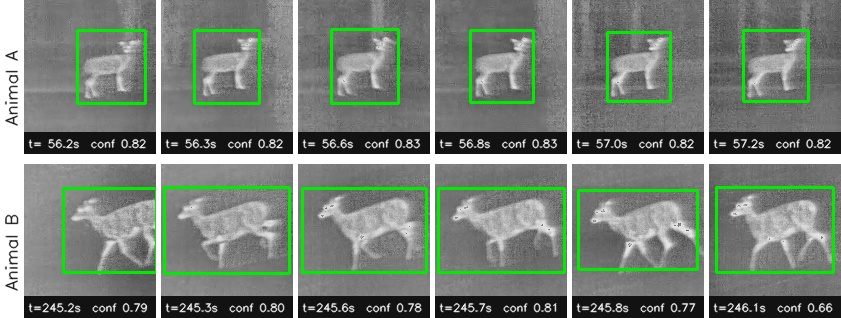
\includegraphics[width=0.75\linewidth]{figures/evidence_two.jpg}
  \caption{\textbf{Per-animal evidence, two individuals.} Every counted animal is exported
  as a contact sheet of its own track, one panel per sampled frame, with the elapsed time
  and the raw per-frame detector confidence beneath each. A human auditor can therefore
  verify any individual count against the frames that produced it. Both animals are from
  videos the detector never trained on. The two rows also show why a per-track score is
  needed: the raw confidence varies by 0.15 across frames of the same animal (Animal B,
  0.66--0.81) even when every frame is a clean detection, so no single frame's value
  characterizes the track.}
  \label{fig:evidence}
\end{figure*}

\subsection{Matching criterion}
\label{sec:criterion}
\label{sec:protocol}

A detection metric asks whether a predicted box \emph{localizes} an animal; a survey asks
whether the animal was \emph{noticed}. On a 27-pixel target these diverge sharply: a box
offset by six pixels falls below IoU 0.5 and is scored as both a false positive and a false
negative, while for counting it has correctly found the animal. We therefore evaluate under
four matching rules --- IoU$\geq$0.50, IoU$\geq$0.30, centre-in-box and \emph{any overlap} ---
and treat the last as the counting criterion, reporting it as presence or counting recall
and never as mAP, with the strict criterion alongside it everywhere.

The criterion is validated against centre-in-box, an independent counting-oriented rule that
accepts a prediction only when its centre falls inside the animal and so rejects oversized
boxes outright. The two agree to within 0.032 F1 across all twelve models, so the
conclusions rest on two criteria agreeing rather than on one being chosen. Precision is
reported alongside recall throughout, which additionally constrains box quality.

\subsection{Decomposing counting error}
\label{sec:decomposition}

The paper's main instrument. Let $G$ be the ground-truth animals in a video and $C$ the
candidate tracks a pipeline produces. For each $g\in G$ we define:

\begin{itemize}\itemsep2pt \parskip0pt
\item \reachedq --- $g$ is touched, on at least one frame, by at least one candidate. If
an animal is not \reachedq, no downstream stage can recover it; this measures
\textbf{detection and tracking}.
\item \primaryq --- among the candidates touching $g$, the one that covers $g$ on the most
frames is not simultaneously the best cover for some other animal. Two animals sharing a
single best-covering candidate are indistinguishable to any decision rule that emits one
count per track; this measures \textbf{association}.
\item \countedq --- the confirmation stage accepted a candidate covering $g$. This measures
\textbf{confirmation}, and it is the end-to-end result.
\end{itemize}

The three are nested, $\countedq \le \primaryq \le \reachedq \le |G|$, and the gaps
attribute error to the three stages. We report all three for every configuration; reporting
only the last, as is conventional, makes a detection failure and a confirmation failure look
identical.

We report mean absolute error in animals per video (MAE), signed bias, and a
\emph{counted} fraction. The latter is $\sum_v \min(\hat{c}_v, c_v) / \sum_v c_v$, capped
per video so that over-counting in one video cannot mask misses in another.

We also report a stricter identity-matched variant, the fraction of individual animals
covered by an \emph{accepted} candidate, which \cref{sec:counting} shows is 10 points
lower; the capped aggregate credits a video for predicting the right \emph{number} even
when the accepted tracks do not land on the animals.

\subsection{Held-out protocol}
\label{sec:heldout}

Counting runs process all 32 videos, but the detector trained on 19 of them, and the
hand-tuned confirmation rule is conventionally swept on the same videos it is reported on.
Both leaks inflate the result. Our protocol closes both: \textbf{sweep the rule on the 19
detector-training videos, freeze it, and report on the 13 unseen videos}. Learned
confirmers are trained and thresholded under the identical split, so the comparison in
\cref{sec:counting} is like-for-like. The protocol is worth 23 points: counting accuracy
measured over all 32 videos is 89.0\%, and on the 13 the detector never saw it is 66.3\%.
